\section{离散化评分}
\label{sec:dep-discretization}

还有一种更朴素的做法：把$X$的取值范围切成几段，$Y$的也切成几段，数一数每个格子里的概率，得到一张有限的概率表，再看这张表离独立有多远。这相当于只在给定的分辨率下观察两个变量。分辨率怎样选、选定以后丢掉了什么，是本节的问题。

设$\{\mathcal{A}_1,\dots,\mathcal{A}_k\}$是$\mathcal{X}$的有限可测划分，$\{\mathcal{B}_1,\dots,\mathcal{B}_l\}$是$\mathcal{Y}$的有限可测划分。记$\alpha(X)$为$X$所在的格子编号，$\beta(Y)$同理。格子标签的联合概率表为
\[
  p_{i,j}=\mathbb{P}\bigl(X\in\mathcal{A}_i,\ Y\in\mathcal{B}_j\bigr),\qquad i=1,\dots,k,\ j=1,\dots,l .
\]
这是一个总体对象：它由联合分布与选定的划分完全确定，与样本无关。

\subsection{固定划分的关联}
\label{sec:dep-fixed-partition}

对格子标签可以用任何离散的依赖度量，最自然的是它们的互信息$I(\alpha(X);\beta(Y))$。$\alpha,\beta$是可测函数，由定理~\ref{thm:dep-mi-invariance}，
\begin{equation}
  I\bigl(\alpha(X);\beta(Y)\bigr)\leq I(X;Y).
  \label{eq:dep-binned-mi-bound}
\end{equation}
离散化只会丢失信息。若一个划分细分了另一个划分，粗格子的标签是细格子标签的函数，再用一次同样的不等式，细划分的互信息不小于粗划分的。

\paragraph{零关联不能反推独立}
固定一个划分得到零互信息，只说明这张表上看不到依赖。连续抛物线$X\sim\operatorname{Unif}(-1,1)$，$Y=X^{2}$给出了反例。在$x=0$处切开$X$，在$y=1/4$处切开$Y$，这是两个边缘各自的中位数。四个格子的概率都可以直接算出：$\{X<0,\,Y<1/4\}=\{-1/2<X<0\}$，概率为$1/4$；其余三个同理，于是
\[
  p_{i,j}=\tfrac14=\tfrac12\cdot\tfrac12,\qquad i,j=1,2 .
\]
这张表恰好是独立的，格子标签的互信息为零，而$X$与$Y$并不独立。原因是$Y$只依赖$\lvert X\rvert$，而$X$的符号与$\lvert X\rvert$独立；在$x=0$处切开，记录的恰好是与$Y$无关的那部分信息。

把$X$的划分加细为四段$[-1,-\frac12)$、$[-\frac12,0)$、$[0,\frac12)$、$[\frac12,1]$，$Y$的划分不变。这时$Y$的格子标签由$X$的格子标签确定：$X$在中间两段时$Y<1/4$，在两端时$Y\geq1/4$。所以条件熵为零，
\[
  I\bigl(\alpha(X);\beta(Y)\bigr)=H\bigl(\beta(Y)\bigr)=\ln2\approx0.693 .
\]
图~\ref{fig:dep-partition-grids}画出这两个划分：同一条抛物线，粗划分下格子概率全为$1/4$，细划分下有四个格子为零。

\begin{BookInlineFigure}
  \centering
  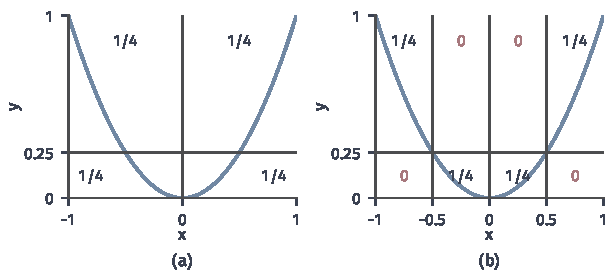
\includegraphics[width=104mm]{figures/07-probability/04-distribution-analysis/matplotlib/dep-partition-grids/figure.pdf}
  \caption{连续抛物线$y=x^{2}$（蓝）在两个固定划分下的格子概率（深灰线为格子边界）。(a)在$x=0$与$y=1/4$处切开，四个格子概率都是$1/4$，标签互信息为$0$；(b)$X$再在$\pm1/2$处切开，八个格子中四个概率为$0$（红），标签互信息为$\ln2$。}
  \label{fig:dep-partition-grids}
\end{BookInlineFigure}

\paragraph{加细的极限}
沿着一列越来越细的划分，标签互信息单调不减，并且不超过$I(X;Y)$。若这列划分最终能分辨所有可测集（例如实轴上以二进端点逐次对分），标签互信息的极限就是$I(X;Y)$；更一般地，互信息等于所有有限划分上标签互信息的上确界\scite{math-cover2006information}。这给出了互信息的另一种读法，也说明了离散化是“从下方逼近”。

在两个边缘都按$k$个等概率区间切分（$k\times k$网格）时，两个例子表现完全不同。对$\rho=0.5$的标准二元高斯，$k=2$时四个格子由象限概率决定，
\[
  \mathbb{P}(X>0,\,Y>0)=\frac14+\frac{\arcsin\rho}{2\pi}=\frac14+\frac{1}{12}=\frac13,
\]
概率表为
\[
  \begin{pmatrix}1/3&1/6\\1/6&1/3\end{pmatrix},\qquad I_2=\tfrac23\ln\tfrac43+\tfrac13\ln\tfrac23\approx0.0566 .
\]
$k$增大时$I_k$迅速上升，$k=8$约为$0.127$，$k=32$约为$0.141$，逼近$0.144$。对连续抛物线，$X$的$k$个等概率区间长为$2/k$，$Y$的$k$个等概率区间对应$\lvert X\rvert$上长为$1/k$的区间。$k$为偶数时，每个$X$格子恰好覆盖两个$Y$格子，且在其中各占一半，所以
\[
  I_k=H\bigl(\beta(Y)\bigr)-H\bigl(\beta(Y)\mid\alpha(X)\bigr)=\ln k-\ln2=\ln\tfrac{k}{2}.
\]
它随$k$无界增长，与定理~\ref{thm:dep-mi-infinite}的无穷大一致；$k=2$给出$0$，正是上面的反例。图~\ref{fig:dep-binned-mi}画出这两条序列。

\begin{BookInlineFigure}
  \centering
  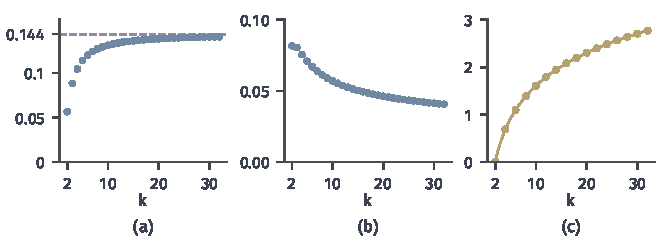
\includegraphics[width=112mm]{figures/07-probability/04-distribution-analysis/matplotlib/dep-binned-mi/figure.pdf}
  \caption{等概率$k\times k$网格上的标签互信息。(a)$\rho=0.5$的标准二元高斯，$I_k$（蓝点）单调上升，逼近紫色虚线$I=0.144$；(b)同一序列除以$\ln k$；(c)连续抛物线，$I_k=\ln(k/2)$（黄，偶数$k$；脚本对$k=4,8$另行数值核对），无界增长。}
  \label{fig:dep-binned-mi}
\end{BookInlineFigure}

\subsection{网格评分}
\label{sec:dep-grid-score}

固定的划分可能恰好错过依赖，自然的补救是在许多划分中搜索，取最能显示关联的那一个。可是互信息随格子数增长，格子越多越占便宜，比较不同大小的网格之前要先归一化。

对实值的$X,Y$，称把$X$的范围切成$k$个区间、$Y$切成$l$个区间所得的划分为一个$k\times l$网格$G$，标签互信息记为$I_G$。标签分别只有$k$与$l$种取值，所以
\[
  I_G\leq\min\bigl(H(\alpha(X)),H(\beta(Y))\bigr)\leq\ln\min(k,l).
\]
于是归一化的比值落在$[0,1]$中。给定格子预算$b\geq4$，定义总体的\term{网格评分}（grid score）
\begin{equation}
  S_b(X,Y)=\sup\Bigl\{\frac{I_G}{\ln\min(k,l)}:\ G\text{为}k\times l\text{网格},\ k,l\geq2,\ kl\leq b\Bigr\}.
  \label{eq:dep-grid-score}
\end{equation}
上确界取遍所有切点位置。令预算$b\to\infty$，得到的总体量就是Reshef等人的\term{最大信息系数}（maximal information coefficient），简称MIC\scite{math-reshef2016dependence}。

\paragraph{零值与确定关系}
总体网格评分的两端可以直接验证。若$X,Y$独立，每个网格的标签都独立，$I_G=0$，评分为零。反过来，若某个预算下评分为零，则所有$2\times2$网格的标签都独立；在$(a,c)$处切开的$2\times2$网格独立，意味着
\[
  \mathbb{P}(X\leq a,\,Y\leq c)=\mathbb{P}(X\leq a)\,\mathbb{P}(Y\leq c),
\]
它对一切$a,c$成立，联合分布函数分解，$X$与$Y$独立。所以只要允许任意切点，网格评分的零值也刻画独立；正是搜索弥补了单个固定划分的缺陷。

另一端，若$Y=f(X)$，$f$在有限个区间上分段连续且单调，$Y$的分布函数连续，则评分在足够大的预算下等于$1$。把$Y$按$l$个等概率区间切分，标签熵为$\ln l$；在单调段的端点与各$Y$切点的原像处切开$X$，每个$Y$格子的原像就是若干个$X$格子之并（对抛物线，取$X$的$2l$个区间即可），这时$Y$的标签由$X$的标签确定，$I_G=\ln l$，而$\min(k,l)=l$，比值为$1$。这与互信息给出$+\infty$形成对照：归一化把“确定关系”压到了上界$1$。

\paragraph{归一化与预算改变刻度}
评分的数值依赖于归一化规则和预算。图~\ref{fig:dep-binned-mi}(b)已经显示，对同一个高斯分布，等概率网格上的$I_k/\ln k$从$k=2$的$0.082$降到$k=32$的$0.041$：分子收敛到$0.144$，分母却继续增长。所以在不同的预算下、或者把分母换成$\ln k$或$\ln(kl)$，得到的是不同的刻度。MIC式的评分把高斯（$I=0.144$）放在$0$与$1$之间某处，把任意无噪声的函数关系都放在$1$，它衡量的是“网格能把关系捕捉得多完整”，不是信息量本身。

\paragraph{总体评分与经验评分}
实际使用时，评分是在一组样本上算的：用$n$个点的经验分布代替联合分布，在预算$b(n)$（常取$n^{0.6}$）以内搜索网格。这样得到的经验评分是另一个对象。即使两个变量独立，有限样本的经验表也不会恰好分解，经验互信息大于零；在许多网格上取最大值，又进一步把偏差放大。

图~\ref{fig:dep-grid-score-sample}用模拟说明这一点。为便于计算，这里只在等频网格中搜索，不优化切点位置，因此它低估了完整搜索的放大效应。对独立的均匀变量，$n=20$时经验评分的平均值约为$0.12$，$95\%$分位数约$0.28$；$n=2560$时平均值降到约$0.019$。对$Y=X^{2}+0.2Z$，$n=20$时经验评分的$5\%$分位数只有约$0.08$，低于独立变量的$95\%$分位数。小样本下两个分布的经验评分大量重叠：一个较高的经验分数，可能只是独立变量在有限样本上的波动。

\begin{BookInlineFigure}
  \centering
  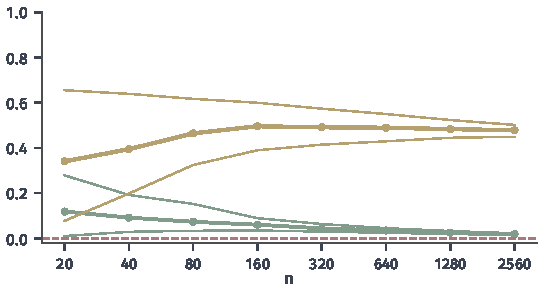
\includegraphics[width=92mm]{figures/07-probability/04-distribution-analysis/matplotlib/dep-grid-score-sample/figure.pdf}
  \caption{经验网格评分随样本量$n$的变化（横轴为对数刻度）。评分在$k,l\geq2$、$kl\leq n^{0.6}$的等频网格上取经验标签互信息除以$\ln\min(k,l)$的最大值。绿：独立的$\operatorname{Unif}(0,1)$对，总体评分为$0$（红色虚线）；黄：$X\sim\operatorname{Unif}(-1,1)$，$Y=X^{2}+0.2Z$。粗线为$200$次重复的平均，细线为$5\%$与$95\%$分位数。种子$719$。}
  \label{fig:dep-grid-score-sample}
\end{BookInlineFigure}

总体网格评分是联合分布的一个确定的泛函；经验评分是样本的函数，带有随机性和偏差。经验网格上的高分，不是“总体关系已经被可靠识别”的证明。要把经验分数变成关于总体的结论，需要分析它在独立假设下的分布并控制多次搜索带来的偏差，这是假设检验的任务，可参考\BookChapterRef{chap:confidence-sets-hypothesis-testing}{卷八第6章“置信集合与假设检验”}。
